%----------------------------------------------------------------------------
\chapter{A rendszer gyakorlati működésének bemutatása} \label{chapter8}
%----------------------------------------------------------------------------

Az alábbiakban szeretném bemutatni az élő arcfelismerés-alapú jelenlétkezelő alkalmazás fő működési folyamatait, a mobilalkalmazásokkal együtt.

Ahhoz, hogy a diák jelenlétét tudja igazolni először is szükség van egy róla készült fotó mentésére, ami szintén a rendszer egyik funkciója. Ezzel a művelettel, kiválasztva a megfelelő szakot, megadva a nevet és Neptun azonosítót, egy kattintásra mentve lesz a kép az erre kijelölt mappába. Ezen mozzanat látható a ~\ref{fig:gy1} ábrán.

\begin{figure}
	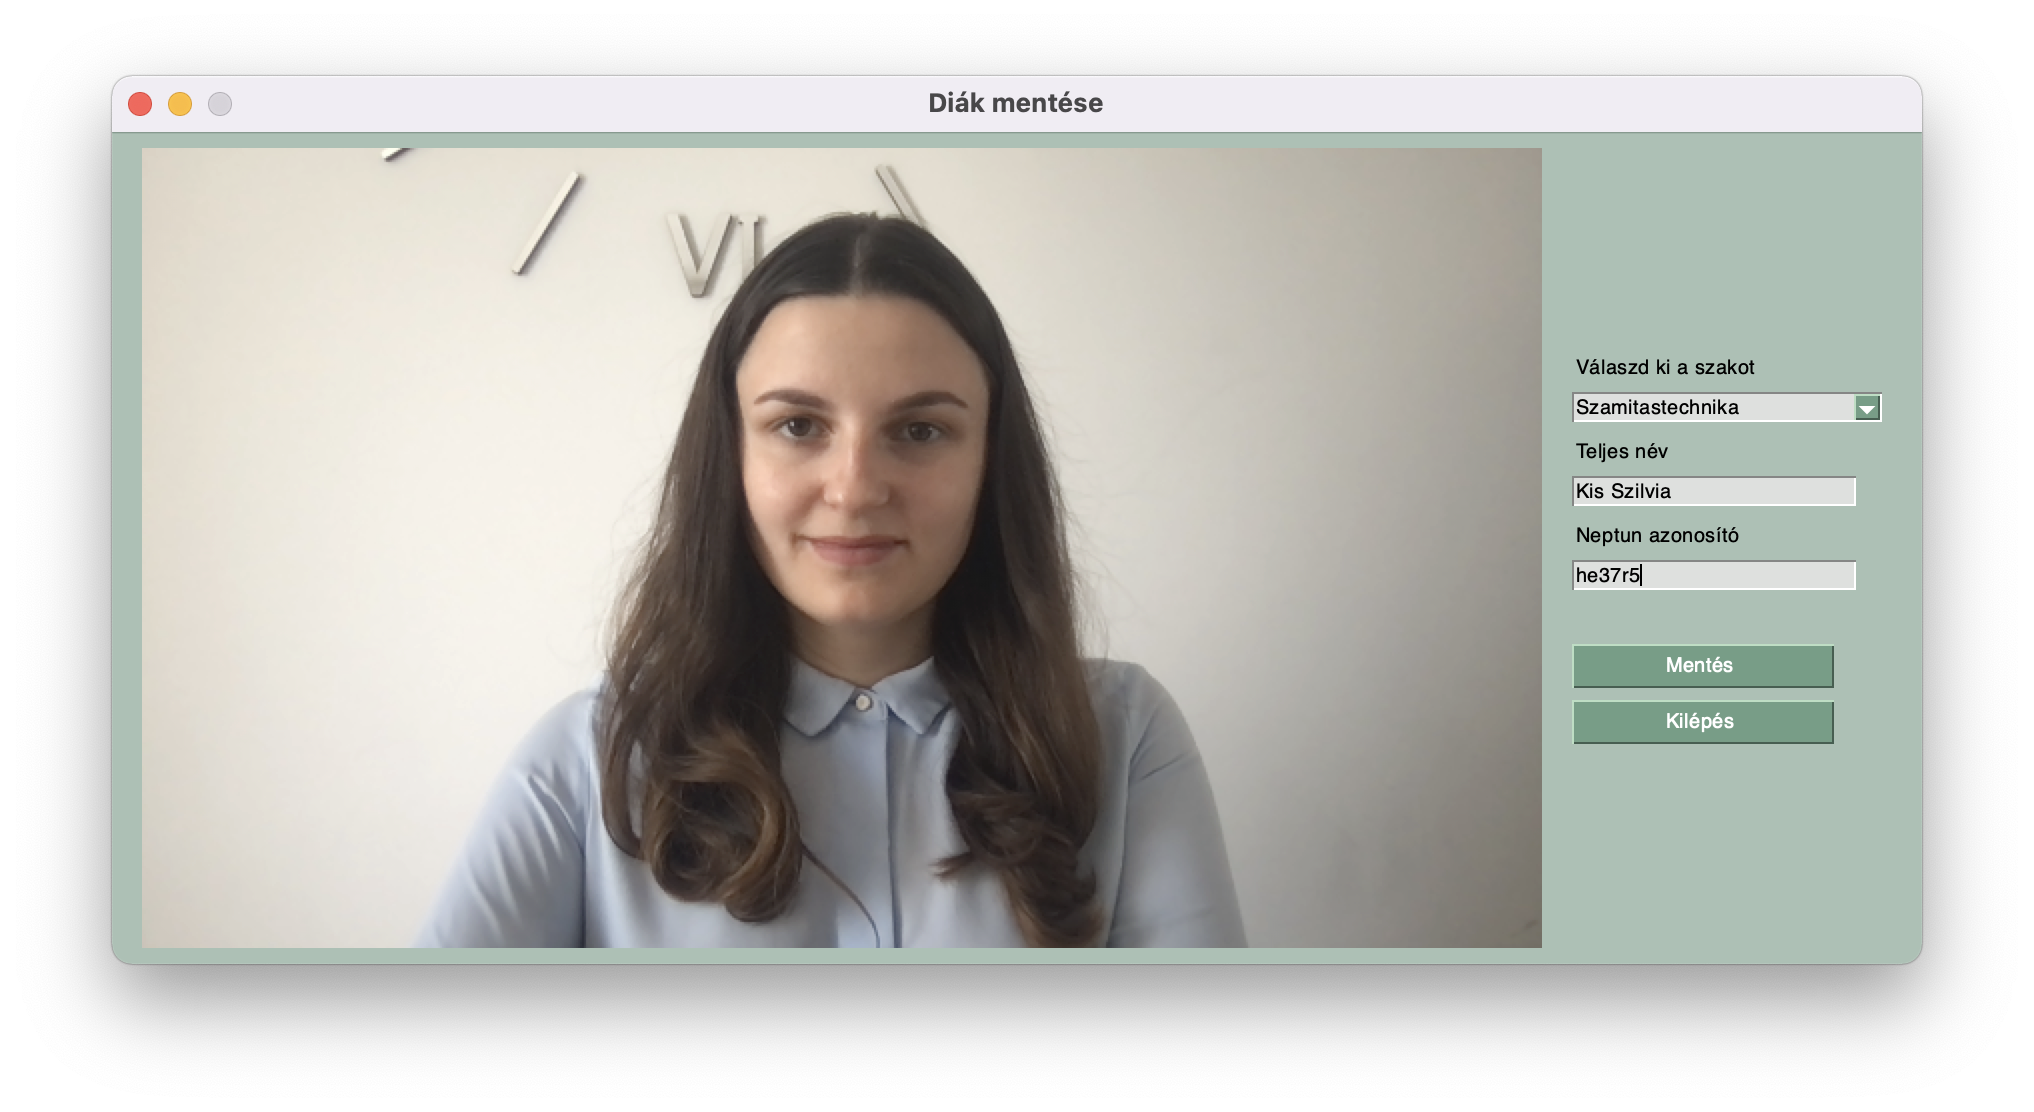
\includegraphics[width=\textwidth]{figures/gy1.png}
	\caption{Diák fényképének mentése}
	\label{fig:gy1}
\end{figure}


Miután minden hallgató bekerült a rendszerbe, indulhat a jelenlétek bevitele. Ehhez csupán annyit kell tenni, hogy a tanár beállítja az órai adatokat, majd a diákok elsétálnak a kamera előtt. Egyszerre akár több diák is azonosítható. A helyes azonosítás végett a képernyőn zöld keret jelenik meg, ahol a név és az életszerűség-érzékelés eredményét is feltüntetjük a könnyen értelmezhetőség kedvéért, ahogy azt a ~\ref{fig:gy2} ábra is mutatja.

\begin{figure}
	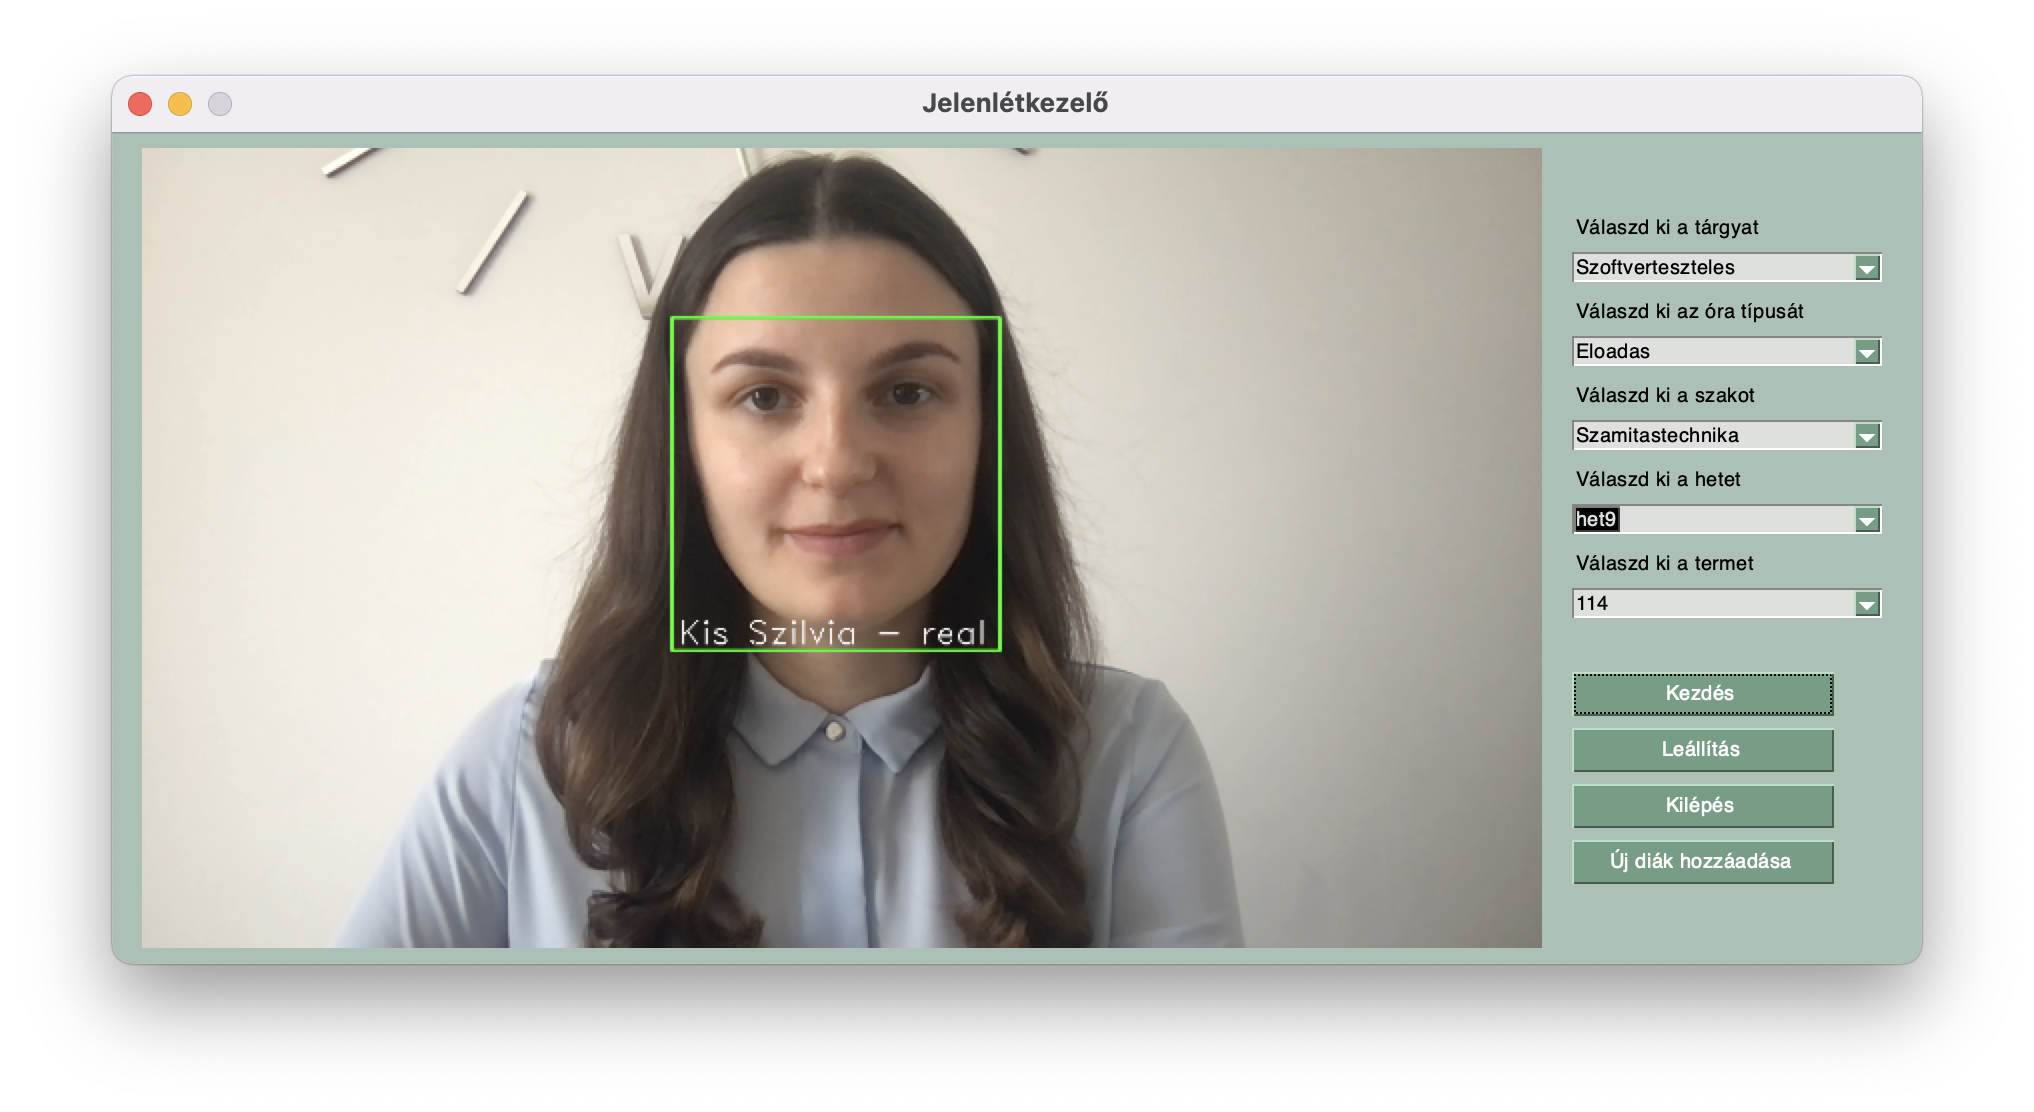
\includegraphics[width=\textwidth]{figures/gy2.png}
	\caption{Jelenlétek bevitele}
	\label{fig:gy2}
\end{figure}

Abban az esetben, ha egy olyan diák szeretné magát azonosítani, akinek adati nem ismertek a jelenlétkezelő alkalmazás részéről, egy \textit{Unknown} felirat jelenik meg, ami egy kattintással orvosolható: \textit{Új diák hozzáadása}. Ezt az esetet szemlélteti a ~\ref{fig:gy3} ábra.

\begin{figure}
	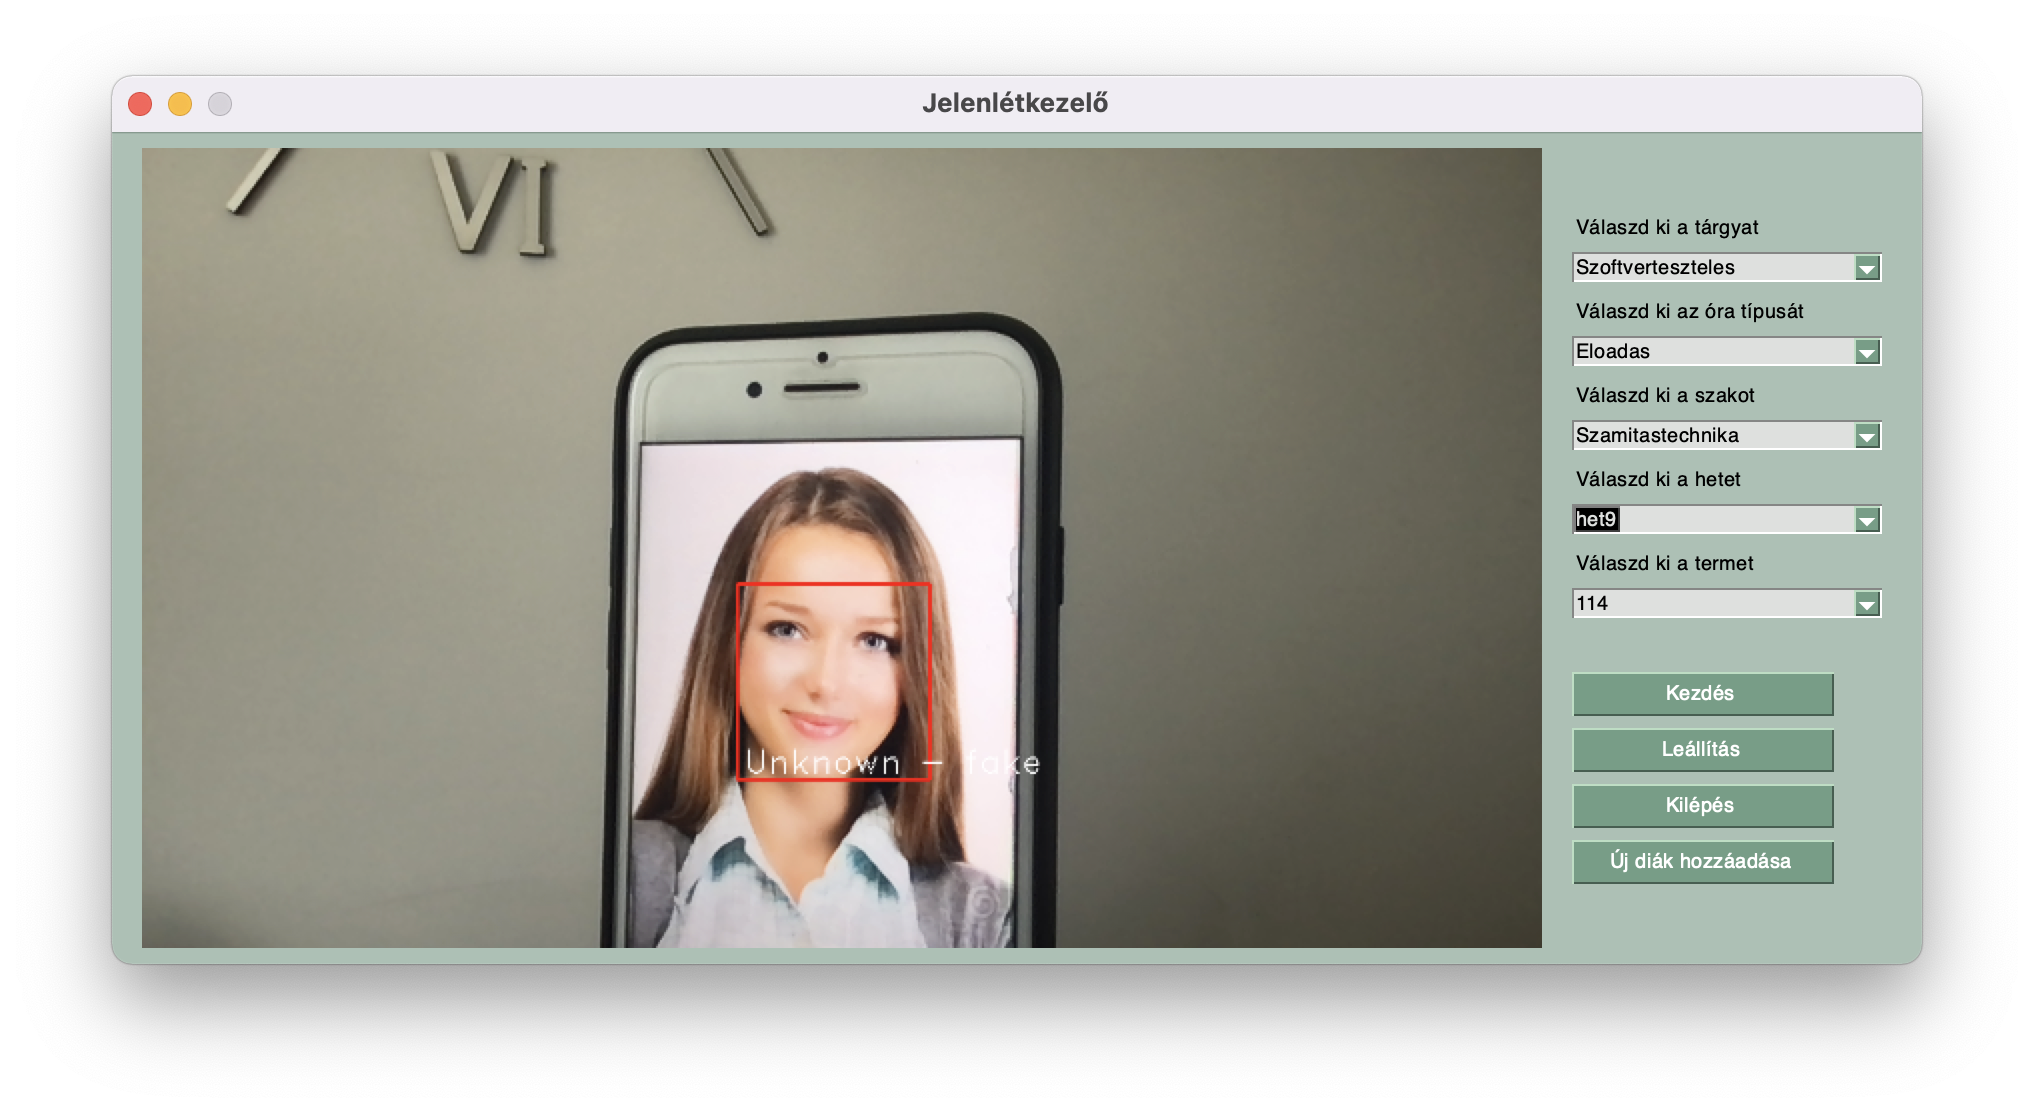
\includegraphics[width=\textwidth]{figures/gy3.png}
	\caption{Ismeretlen arc észlelése}
	\label{fig:gy3}
\end{figure}

A dolgozat fő kutatási témája az életszerűség-érzékelés, fő szerepet játszik a szoftver működésében, ugyanis ez az algoritmus felel a megbízhatóságért. Ez az jelenti, hogy a rendszert nem lehet olyan módszerekkel kijátszani, mint például egy másik diák fényképének mutatása akár fizikai fényképről vagy egy digitális eszközről. Abban az esetben ha a rendszer egy \enquote{hamis}, azaz nem élő arcot detektál, piros kerettel és a megfelelő felirattal jelzi ezt, amint az a ~\ref{fig:gy4} ábrán is látható.

\begin{figure}
	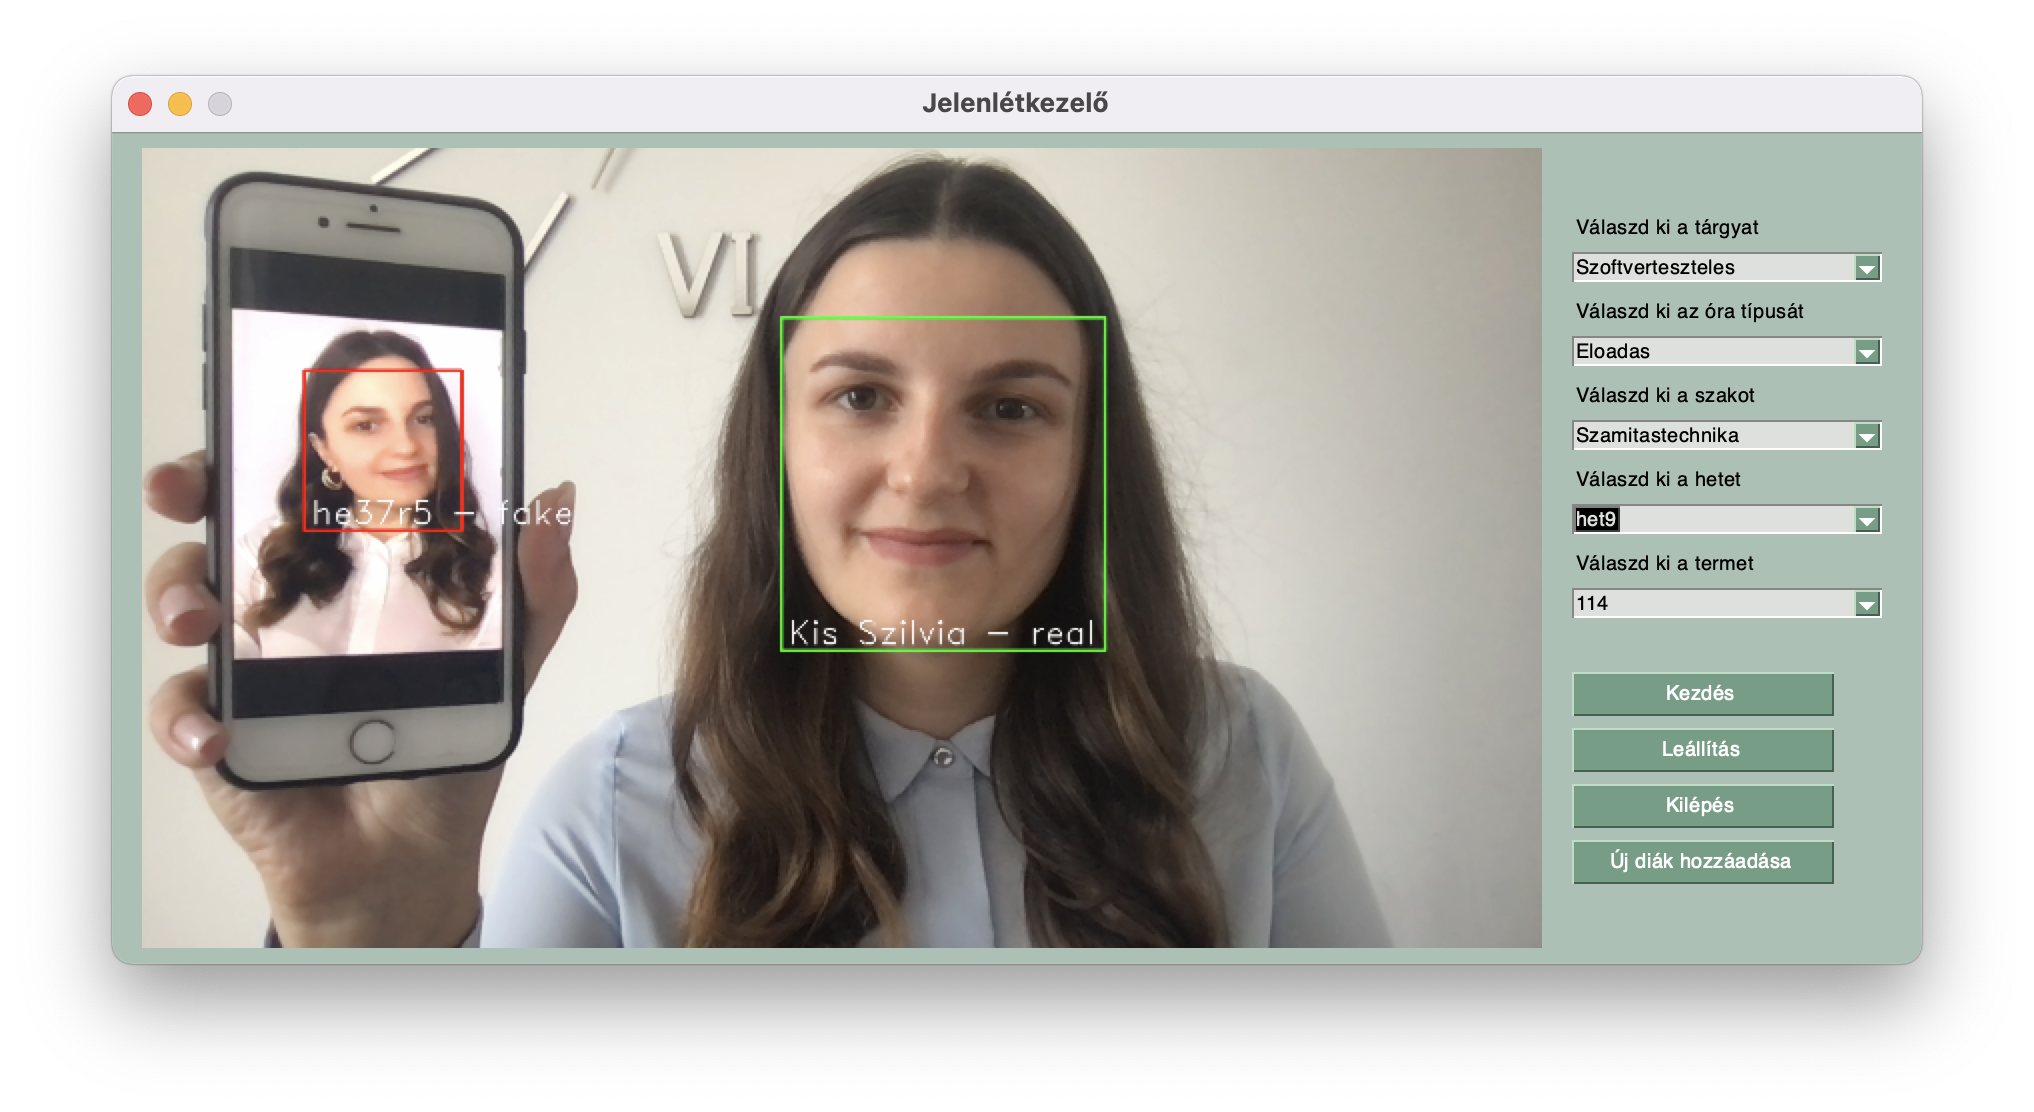
\includegraphics[width=\textwidth]{figures/gy4.png}
	\caption{Hamis és élő arc detektálása egyidejüleg}
	\label{fig:gy4}
\end{figure}

\newpage


Ezt követően minden olyan hallgató jelenléte, akit a rendszer detektált, bekerül az adatbázisba. Mivel egy adatbázist használunk mind az arcfelismerő és életszerűség-érzékelő modul, mind pedig a mobilalkalmazások esetében, a kapcsolat egyszerű. Az arcfelismerő és életszerűség-érzékelő modul beírja a jelenléteket, a mobilapplikáció pedig lekéri és megjeleníti azokat.

Fontos megjegyeznünk, hogy a mobilapp letöléltése nem kötelező. Abban az esetben ha a diák mégis használni szeretné a jelenlétek utánkövetése végett, szükséges egy regisztráció, amit megerősítve be tud lépni az alkalmazásba. A tanár szerepkörű felhasználóra ugyanez érvényes, ám esetükben egy hasznos funkció, a jelenlétek kimentése végett javasolt a mobilalkalmazás használata. 

Fő funkciónak számít a Tanár applikáció esetében is a jelenlétek megtekintésének lehetősége. Ezt a lépéssorozatot ábrázolja a ~\ref{fig:gy5} ábra. Emmellett ugyanolyan fontos a jelenlétek kimentése, választott formátumban. Ebben az esetben a jelenlétek letöltésre kerülnek az eszközre, szakora és az óra típusára lebontva. A letöltés folyamata a ~\ref{fig:gy6} ábrán látható.

A Diák alkalmazás esetén a jelenlétek megtekintése a ~\ref{fig:gy7} ábrán bemutatott procedúra alapján történik.

Ezenkívül minden kisegítő funkció ugyanúgy elérhető az alkalmazásokon belül, legyen az e-mail küldés, naptáresemény létrehozása vagy épp a Google tanterembe való belépés lehetősége.



\begin{figure}[htbp]
	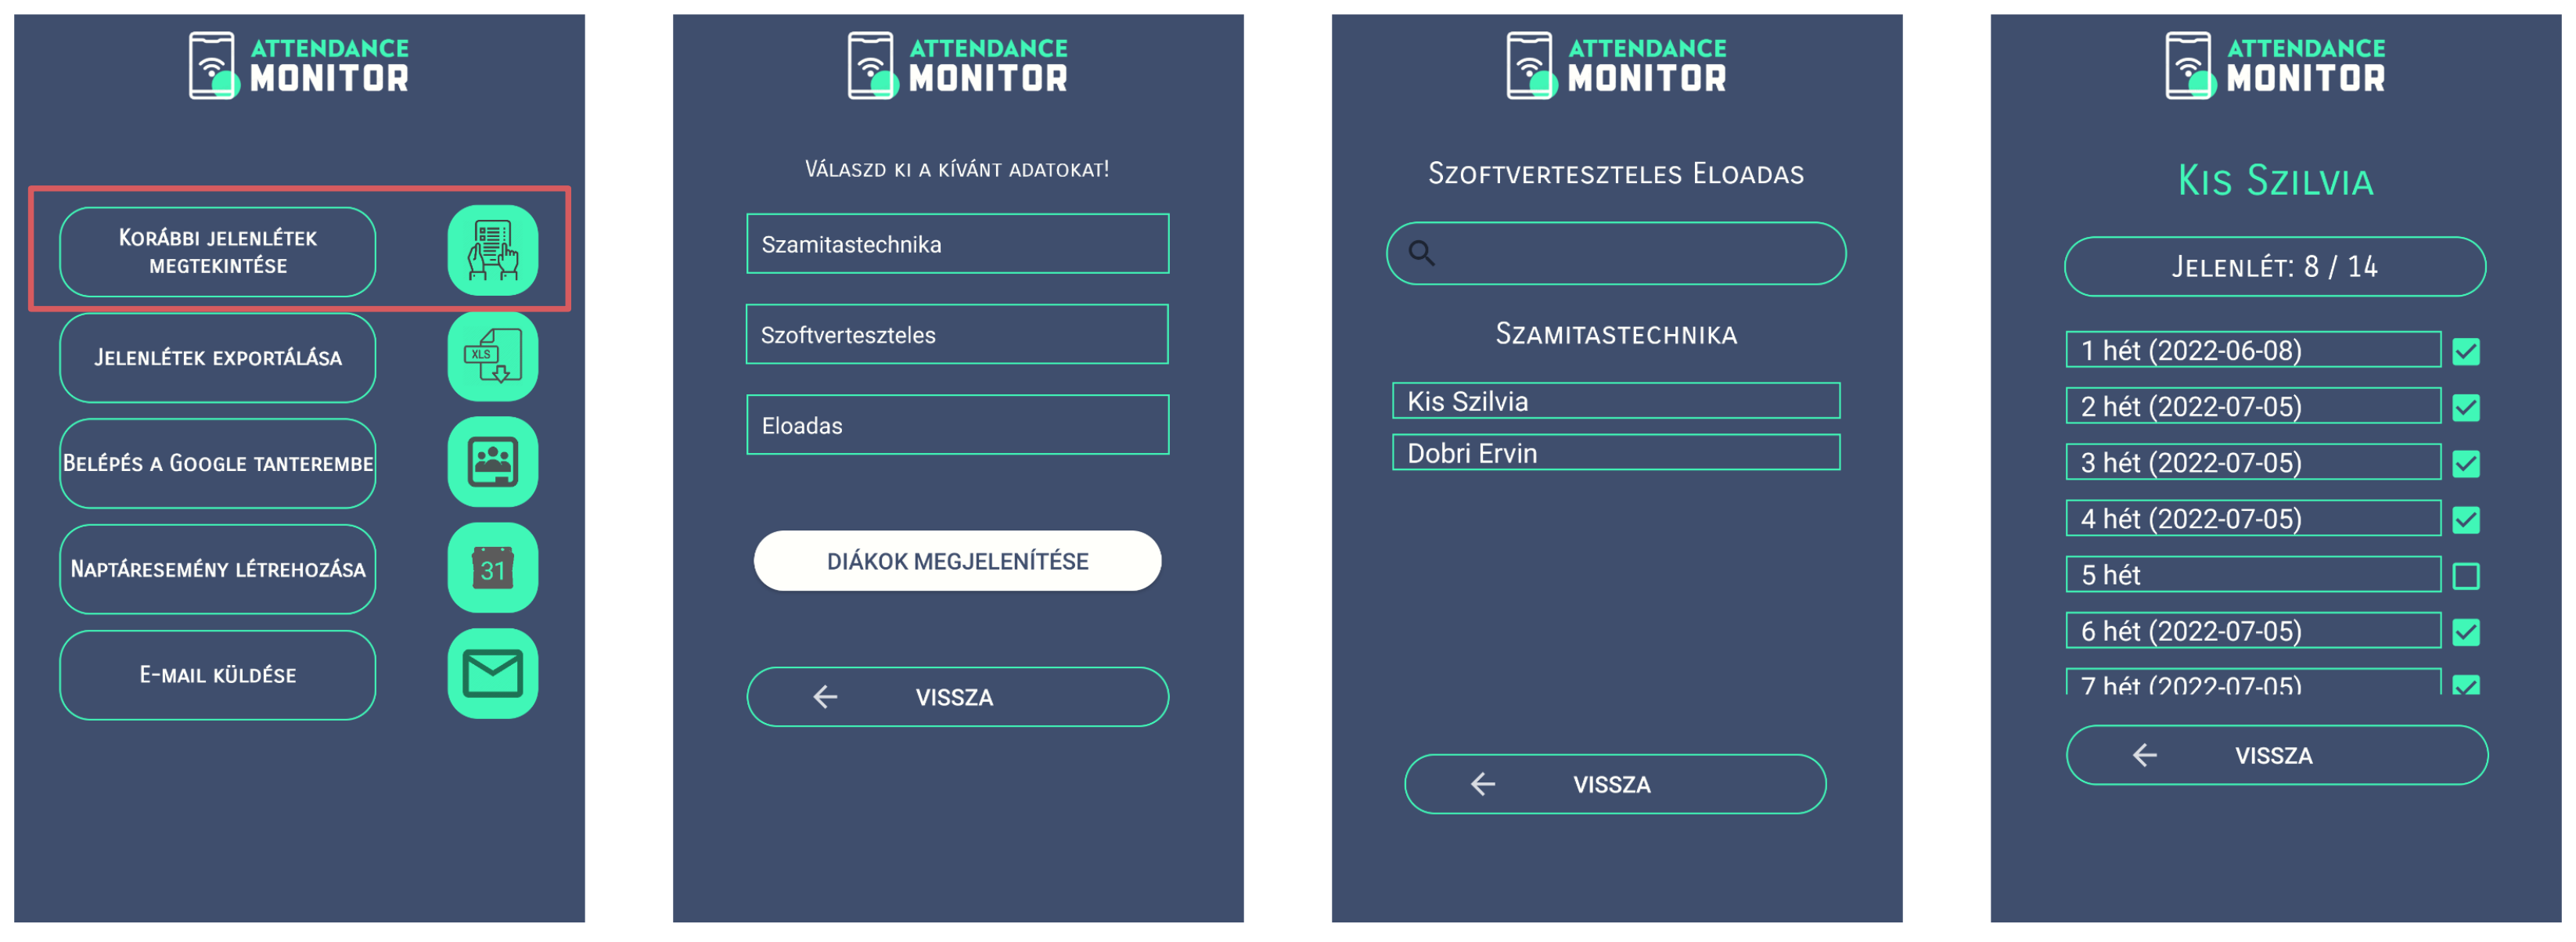
\includegraphics[width=\textwidth]{figures/gy5.png}
	\caption{Jelenlétek megtekintése a Tanár applikációban}
	\label{fig:gy5}
\end{figure}

\begin{figure}
	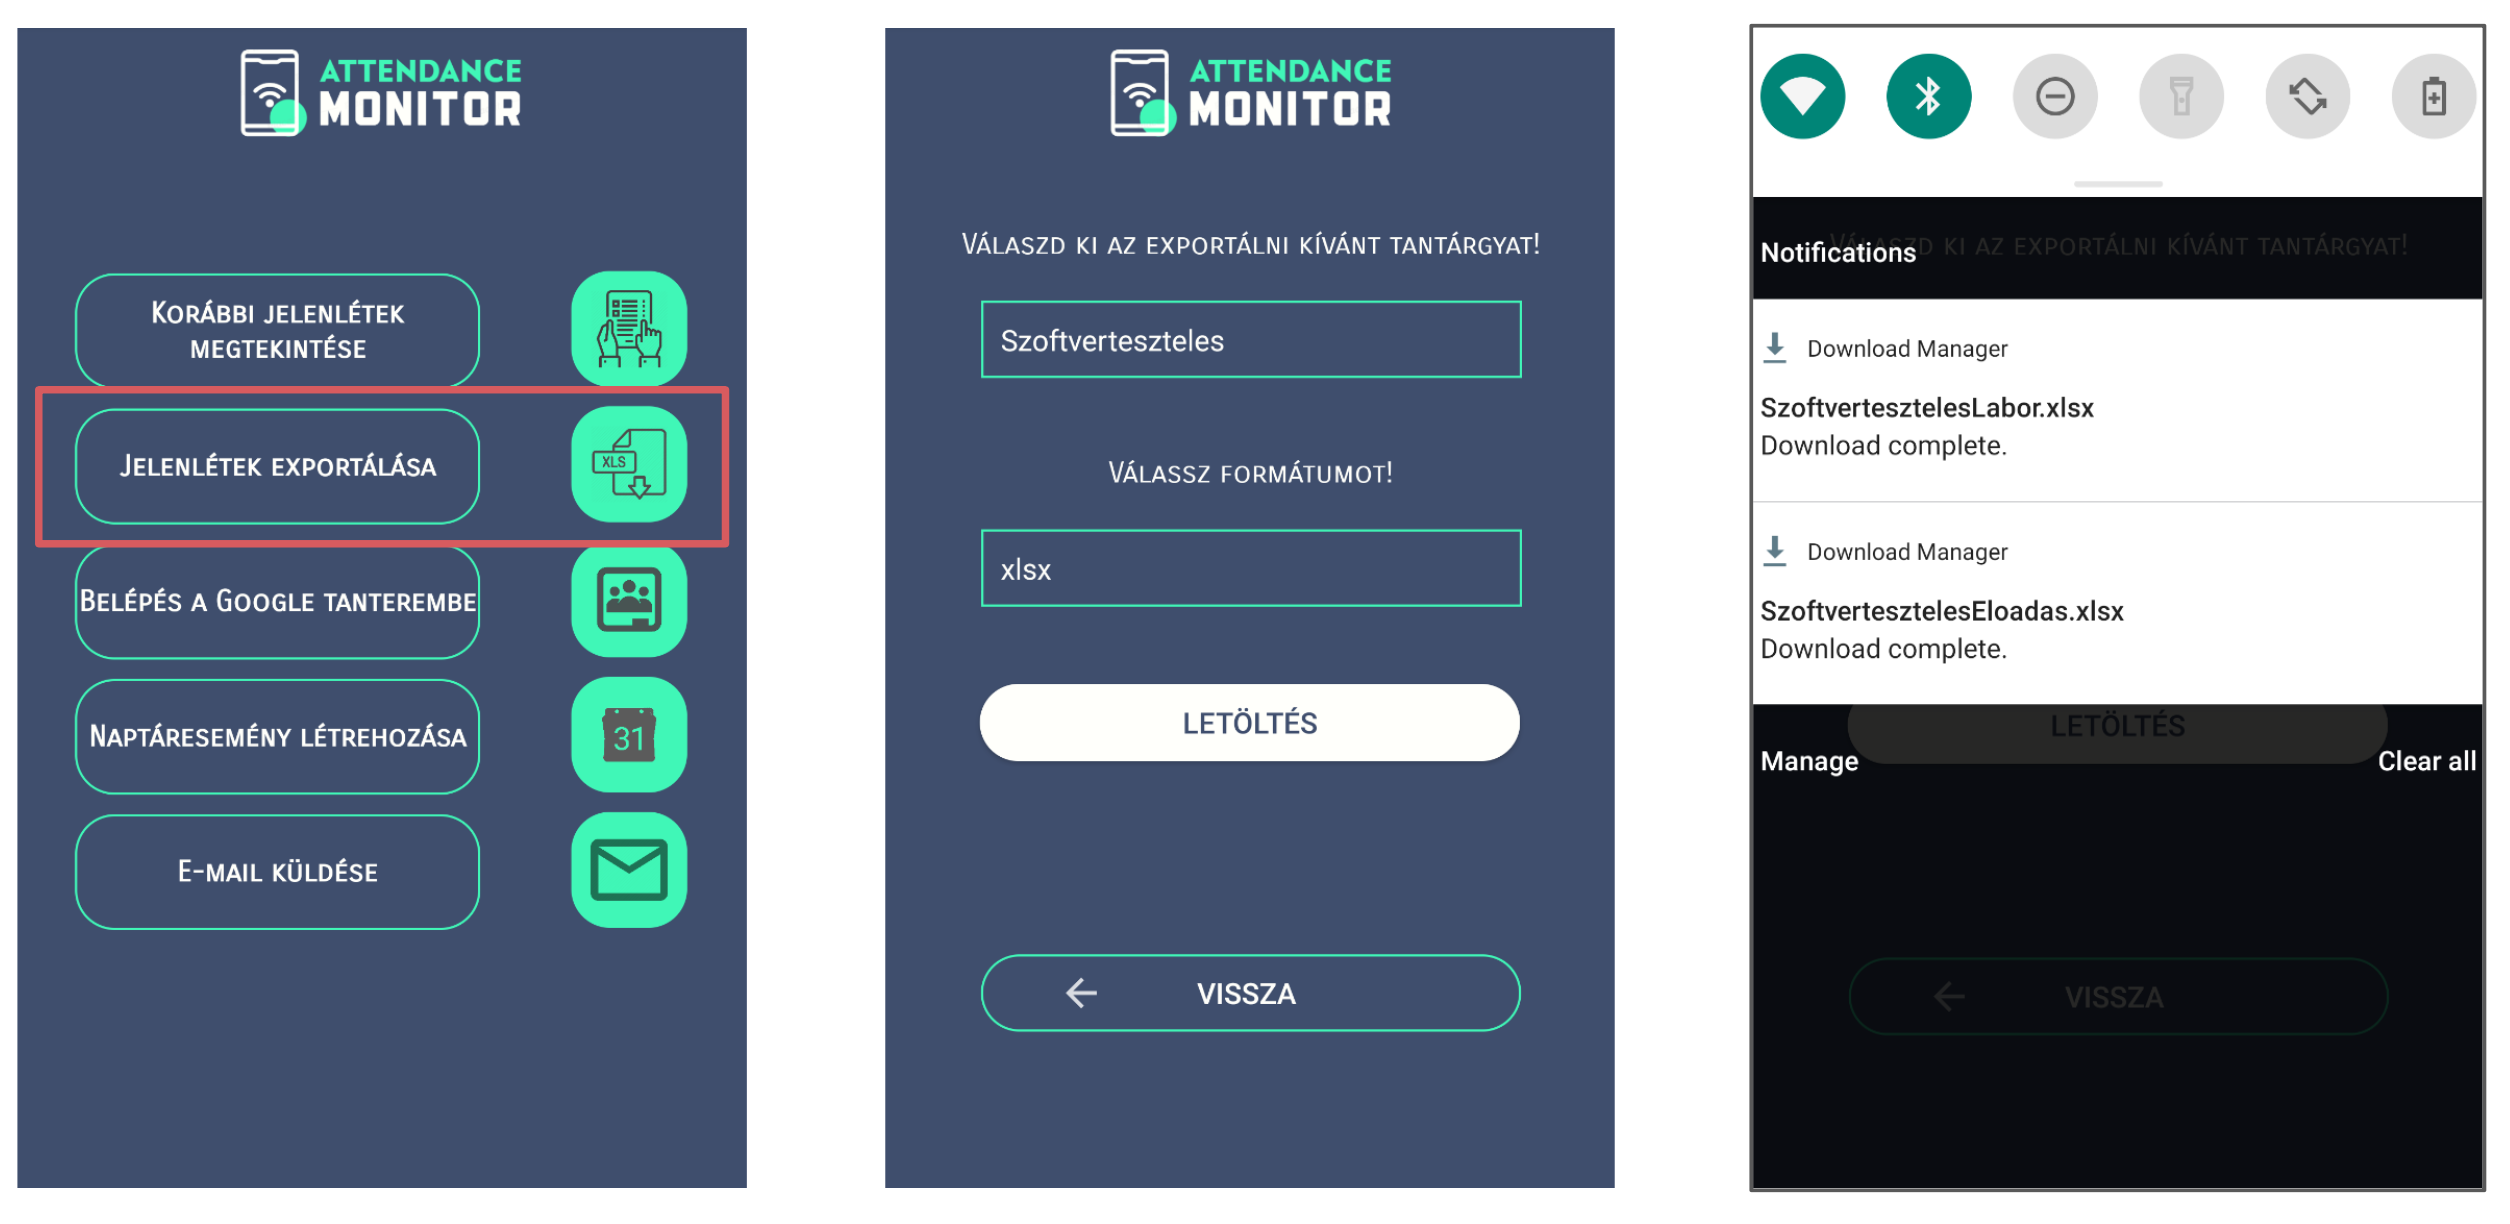
\includegraphics[width=\textwidth]{figures/gy6.png}
	\caption{Jelenlétek letöltése a Tanár applikációban}
	\label{fig:gy6}
\end{figure}

\begin{figure}
	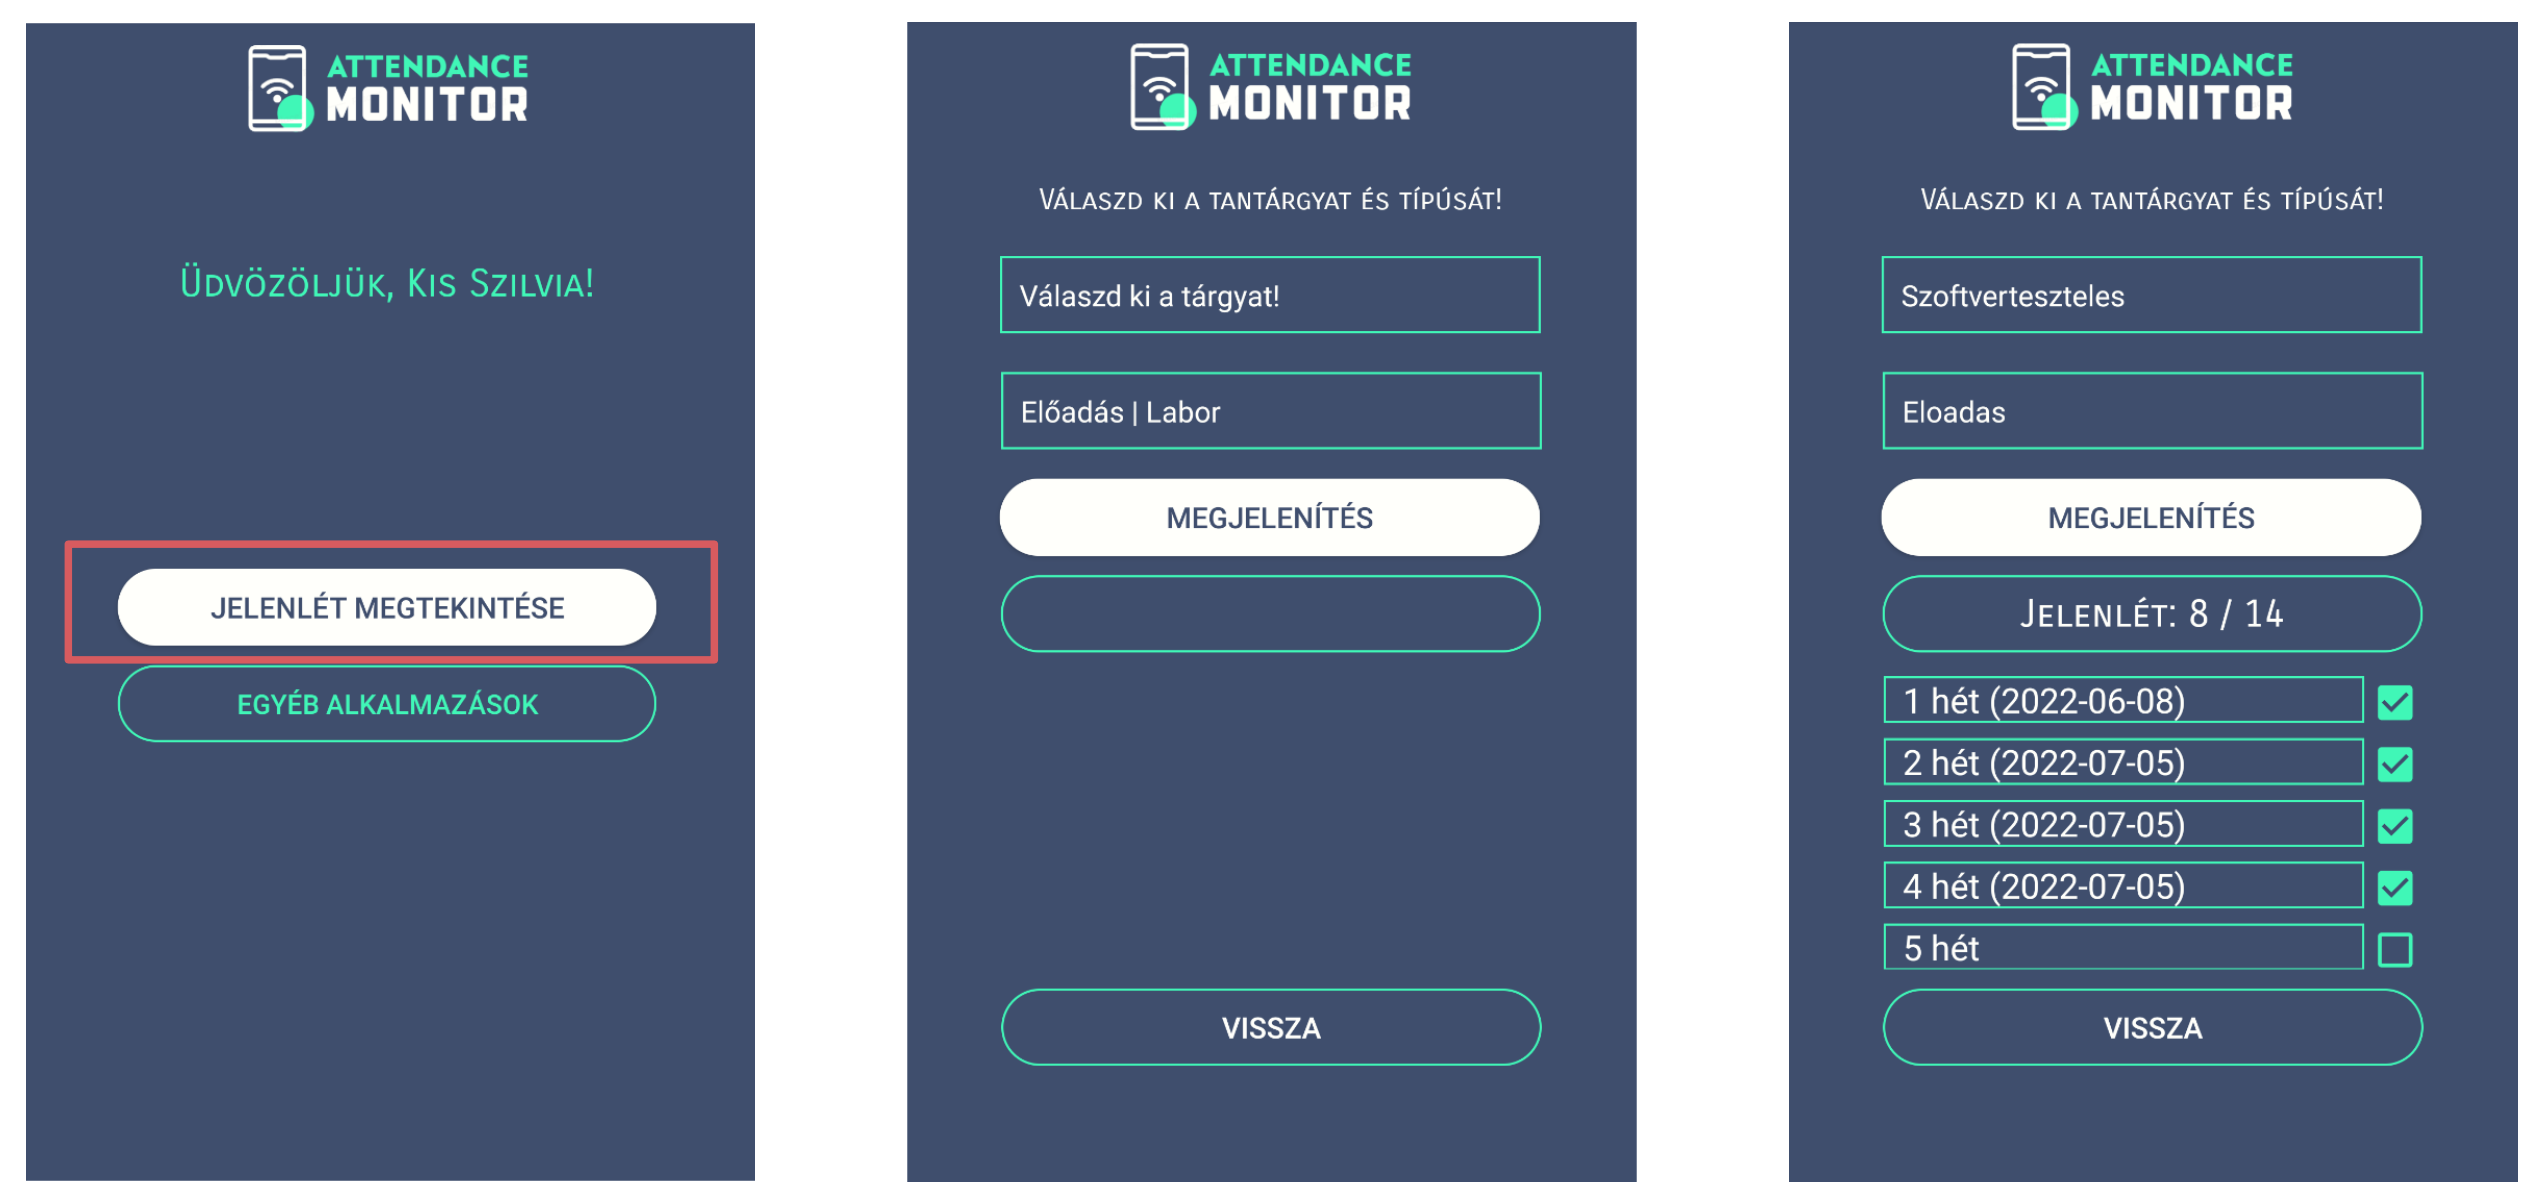
\includegraphics[width=\textwidth]{figures/gy7.png}
	\caption{Jelenlétek megtekintése a Diák applikációban}
	\label{fig:gy7}
\end{figure}